% ===================================================================
% Supplementary Material --- v2 diffusion-based inverse-RG model
% Paste into your paper where the appendix/supplementary section goes.
% Assumes: \usepackage{graphicx}, \usepackage{amsmath}, \usepackage{amssymb},
%          \usepackage{booktabs}
% Images expected at figures/01_ladder_drift.png ... figures/19_ess_weights.png
% ===================================================================

\section{Supplementary Material --- v2 Model}
\label{sec:appendix-v2}

This appendix documents the v2 checkpoint of the diffusion-based inverse-RG
sampler for 2D compact U(1) lattice gauge theory. It addresses four
questions: (1) does the generated ensemble match exact results, inside and
far outside the training range; (2) how does the sampler compare, in
wall-clock cost and correctness, against the strongest classical baseline we
could construct (instanton-update HMC, whose global $Q$-hop is the
volume-independent uniform $Q$-shift move); (3) what a diffusion-generated
configuration buys as an HMC starting point; and (4) what an
exact-likelihood diagnostic honestly says about the model as an
importance-sampling proposal.

\subsection{Methodology}
\label{sec:appendix-v2-methods}

\paragraph{The model.} A gauge-covariant score network (invariant
plaquette/rectangle inputs, plaquette-curl output head, per-site channel
normalization) is trained by denoising score matching on wrapped link angles
$\theta \in (-\pi,\pi]$, conditioned on the $2\times 2$-blocked coarse
field, over continuous log-uniform couplings $\beta \in [1, 60]$ at
$L = 8, 16, 32$. Generation runs the reverse process as one inverse-RG step
(coarse $\beta_c$ at $L$ $\to$ fine $\beta_f$ at $2L$, matched so the
blocked fine theory reproduces the coarse one). Relative to the previous
(v6) checkpoint, v2 adds: exact-symmetry data augmentation ($90^\circ$
rotations, reflections, and charge conjugation $\theta \to -\theta$, which
enforces $P(Q) = P(-Q)$ statistically); oversampling of small noise levels
at high $\beta$ (targeting the $\sigma$-region that resolves the narrow
high-$\beta$ link distributions); a per-site normalization with no
lattice-size dependence; a global coarse-FiLM channel carrying the coarse
winding sum $2\pi Q/V$ to every layer; and a $\beta$-gated exact-score
blend (analytic noised-Wilson score as $\sigma \to 0$, gated off below
$\beta \approx 5$).

\paragraph{Honesty conventions.} All topology results use the strict
setting: rethermalization performs \emph{no} topological (instanton-hop)
updates, so the model plus the deterministic coarse-charge transport must
carry the sector --- rethermalization cannot manufacture topology. Raw
(pre-enforcement) topology metrics are quoted where model transport itself
is at issue. Error bars are per-chain time averages (never pooled across
time $\times$ chain) for HMC series, and per-config SEM for generated
ensembles; $z$-scores are against exact character-expansion values. Two
independent seeds were run for the out-of-sample tracks; all seed-2 results
confirmed seed-1 within statistics.

\paragraph{Statistical baseline.} Under these conventions the v2 checkpoint
matches exact results across 38 study cases from $\beta_f = 1.49$ to
$872.8$ ($15\times$ the training maximum) and volumes to $L = 128$
($64\times$ the training area), with topology transport improved over v6
(mean raw spurious $\langle Q^2 \rangle$ excess $5.3 \to 2.9$; raw
charge-match rate $0.17 \to 0.21$) at equal Wilson-observable accuracy.

% -------------------------------------------------------------------

\begin{figure}[p]
  \centering
  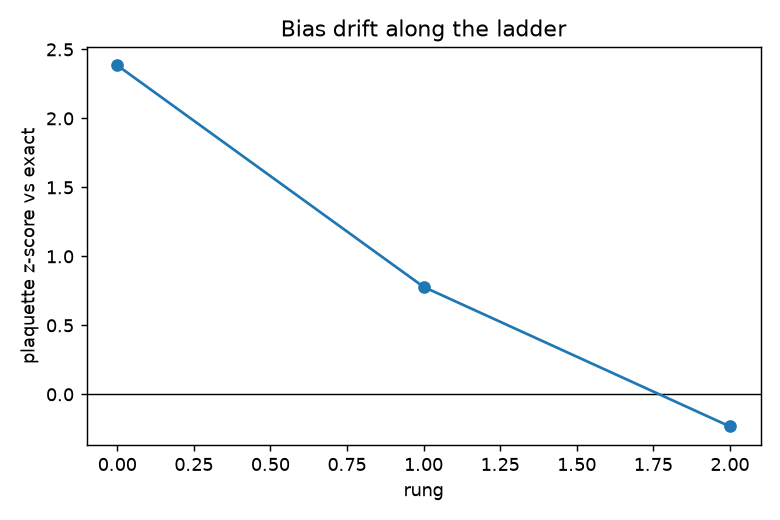
\includegraphics[width=0.9\linewidth]{figures/01_ladder_drift.png}
  \caption{\textbf{Ladder observable drift.} Mean plaquette (and companion
  observables) at each rung of the iterated ladder $L = 8 \to 16 \to 32 \to
  64$ ($\beta = 1.35 \to 4.0 \to 14.15 \to 55.02$), generated ensemble vs
  exact. Drift does not accumulate across rungs: each inverse step is
  followed by short local rethermalization (16 sweeps, no $Q$-hops), which
  pins the UV before the next doubling.}
\end{figure}

\begin{figure}[p]
  \centering
  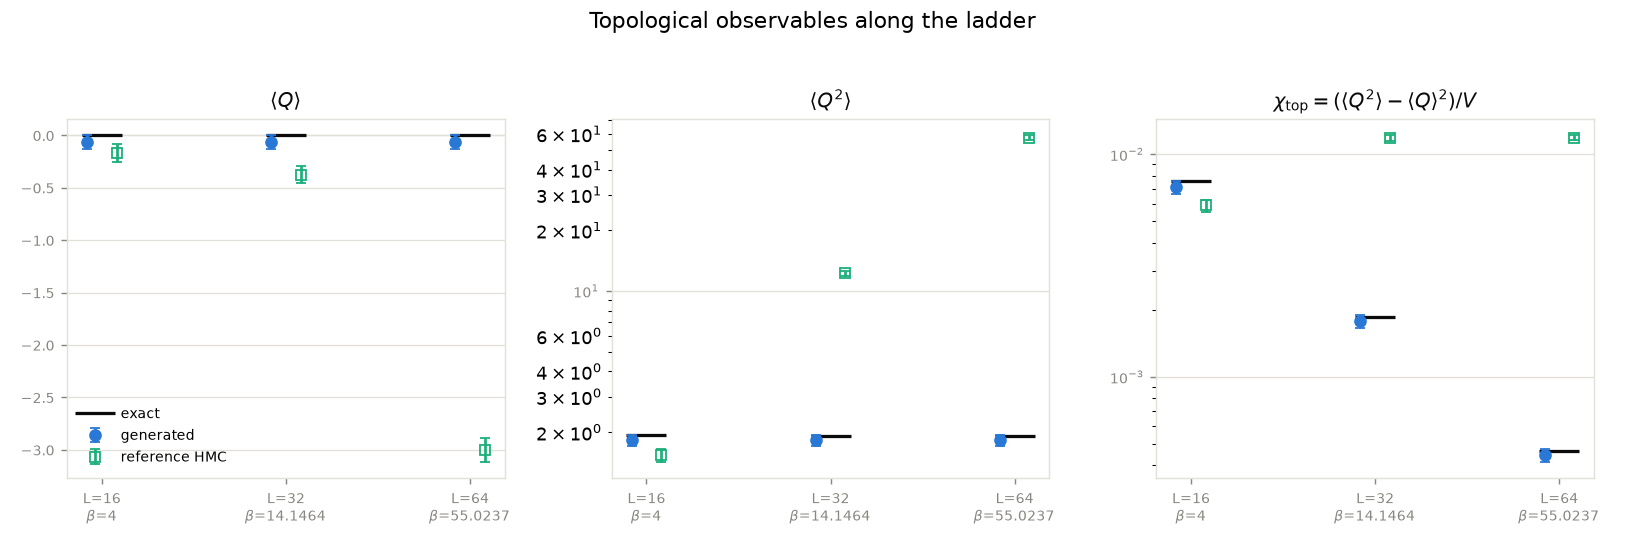
\includegraphics[width=0.9\linewidth]{figures/02_ladder_topology.png}
  \caption{\textbf{Ladder topology.} Topological charge distribution by rung
  against the exact finite-volume $P(Q)$. The sector content is inherited
  from the coarse base --- an $L = 8$, $\beta = 1.35$ ensemble where HMC
  tunnels freely --- and transported structurally up the ladder, which is
  how correct $\langle Q^2 \rangle$ persists at couplings where any direct
  chain is frozen.}
\end{figure}

\begin{figure}[p]
  \centering
  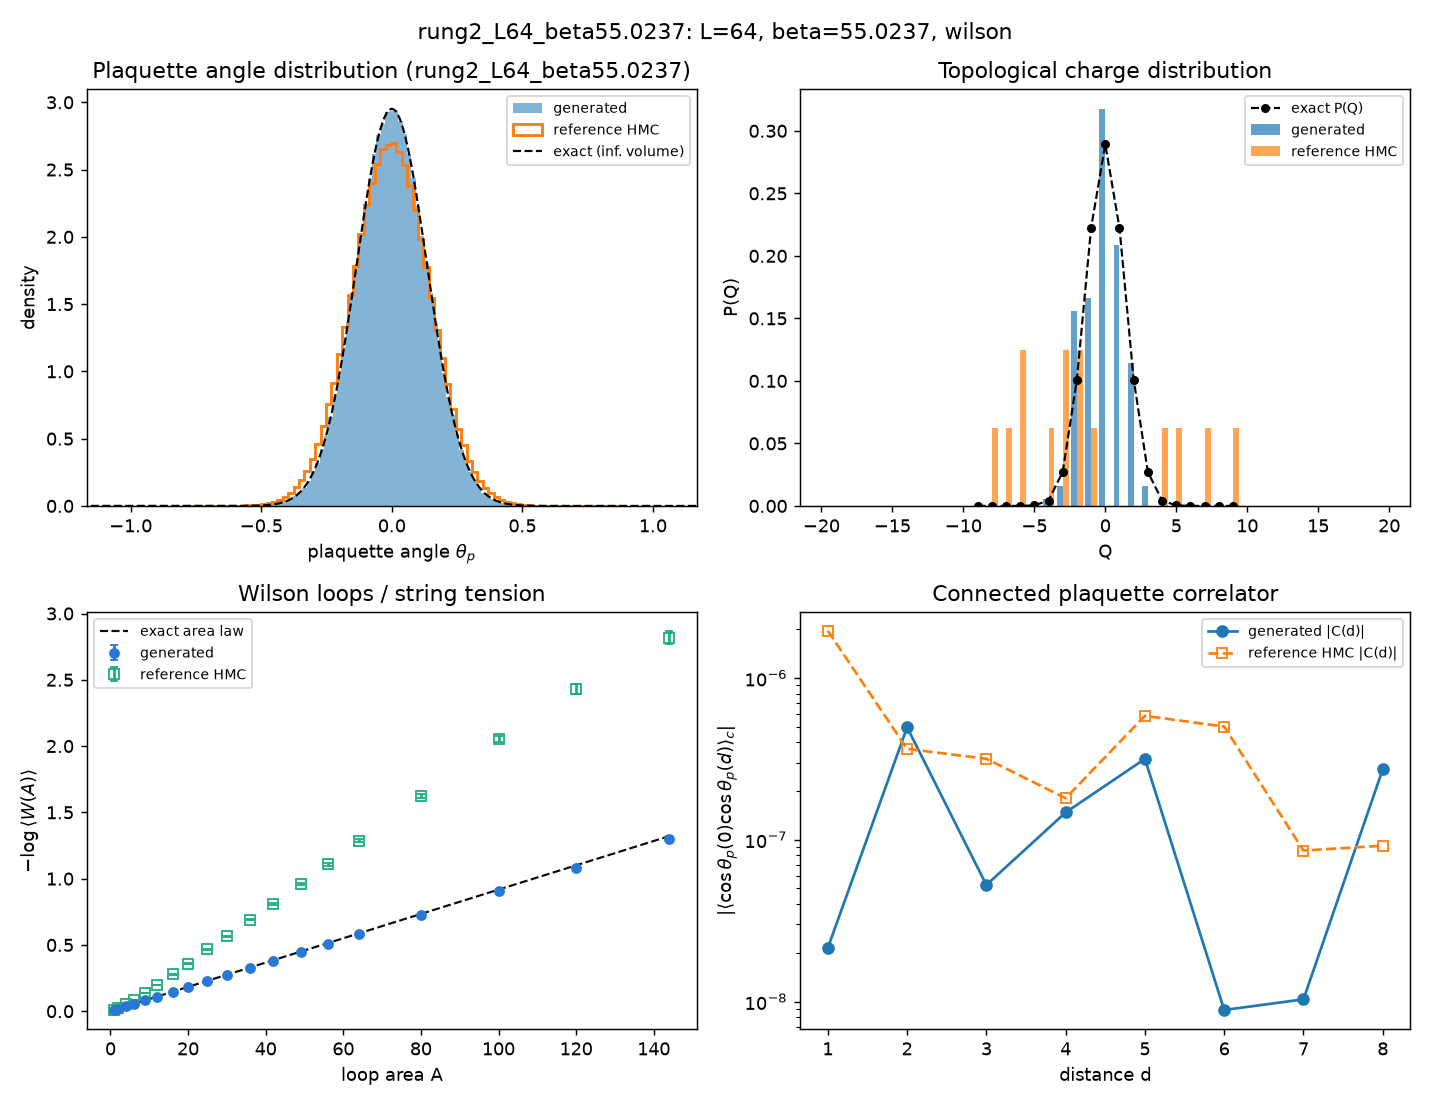
\includegraphics[width=0.9\linewidth]{figures/03_ladder_rung_L64.png}
  \caption{\textbf{Top rung validation ($L = 64$, $\beta = 55.02$).} Full
  observable panel at the ladder's final rung: plaquette and Wilson-loop
  distributions, $Q$ histogram vs exact $P(Q)$. This coupling/volume is far
  beyond anything in the training data.}
\end{figure}

\begin{figure}[p]
  \centering
  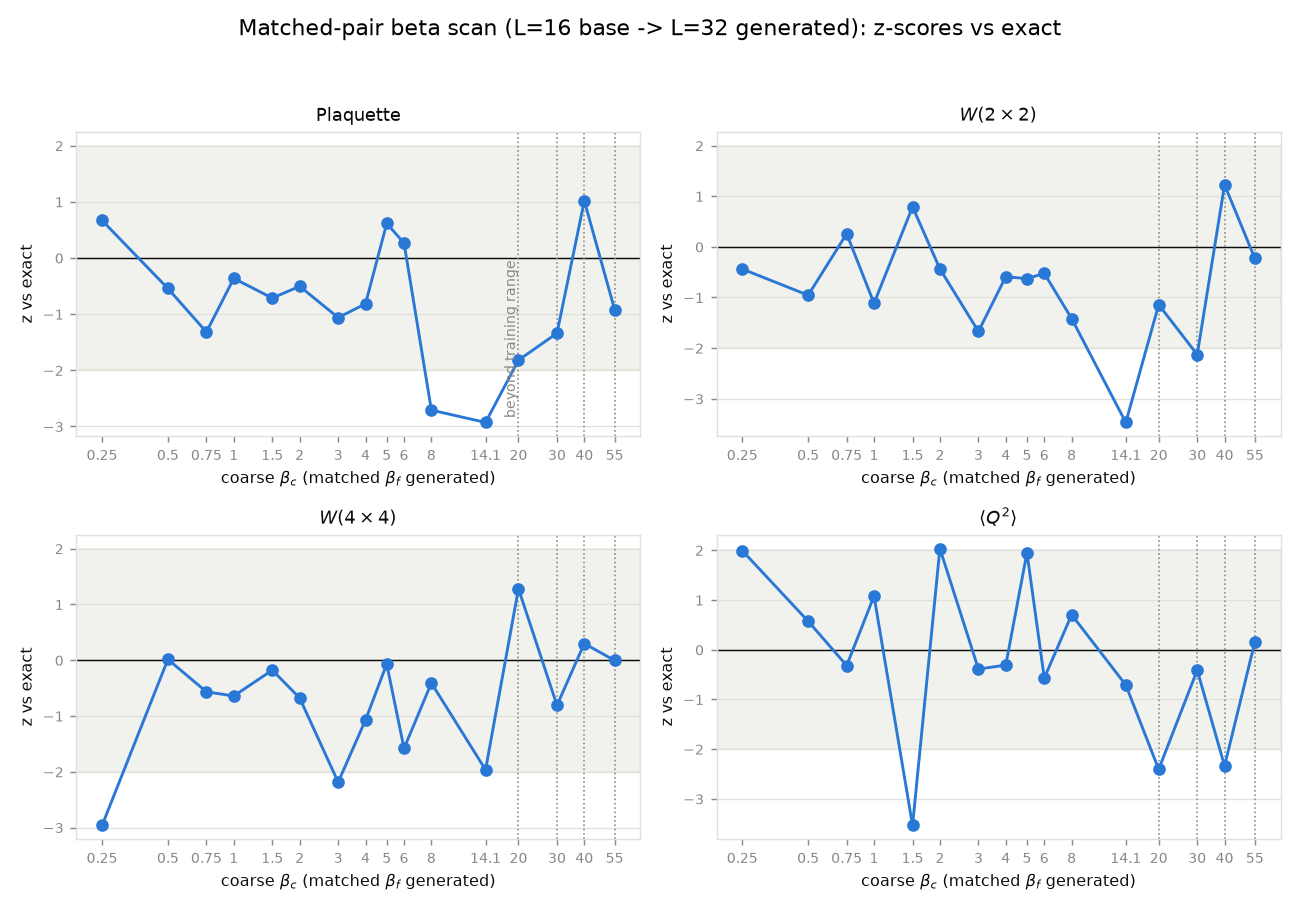
\includegraphics[width=0.9\linewidth]{figures/04_matched_scan.png}
  \caption{\textbf{Matched-pair coupling scan (parts A and D).} One inverse
  step $L = 16 \to 32$ per case over $\beta_f = 1.49$--$218.58$ (matched
  pairs), generated vs exact: $z$-scores stay within the $|z| \le 2$--$3$
  statistical band over more than two decades of coupling, from a single
  checkpoint with no per-case tuning.}
\end{figure}

\begin{figure}[p]
  \centering
  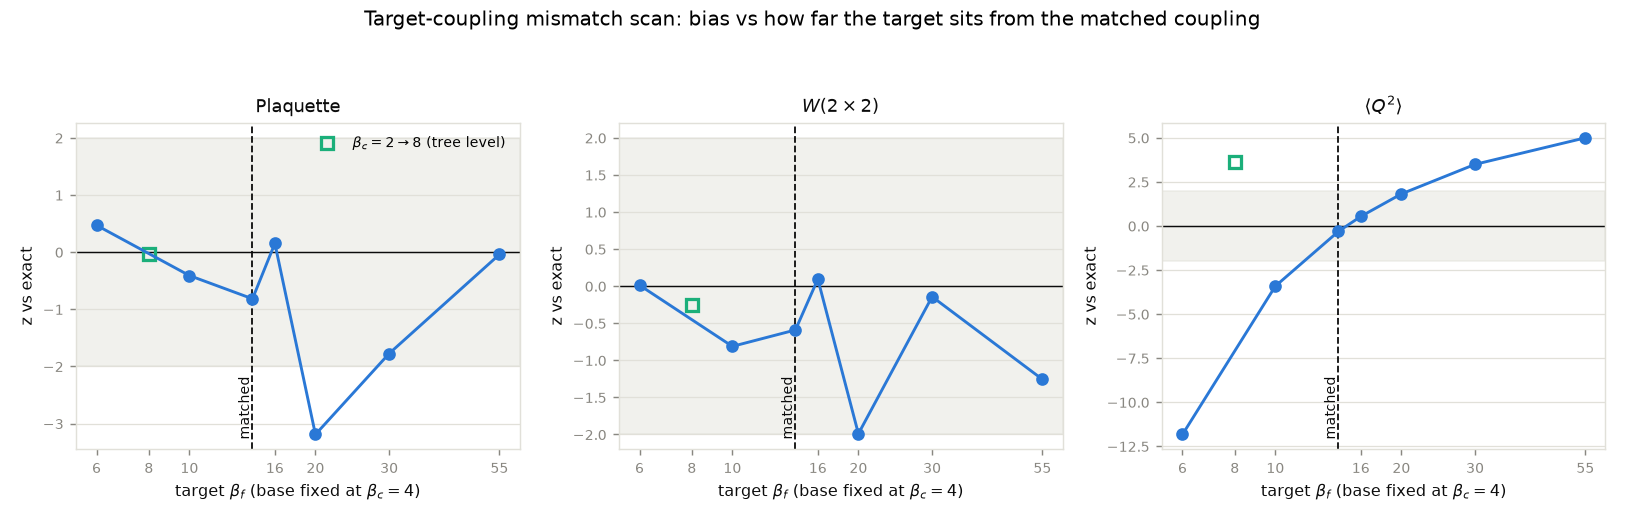
\includegraphics[width=0.9\linewidth]{figures/05_mismatch_scan.png}
  \caption{\textbf{Deliberate mismatch controls (part B).} The conditioning
  coarse ensemble is held at $\beta_c = 4$ while the target $\beta_f$ is
  varied off the matched value. The model tracks the \emph{requested}
  coupling --- evidence that $\beta$-conditioning, not the coarse input
  alone, sets the generated physics.}
\end{figure}

\begin{figure}[p]
  \centering
  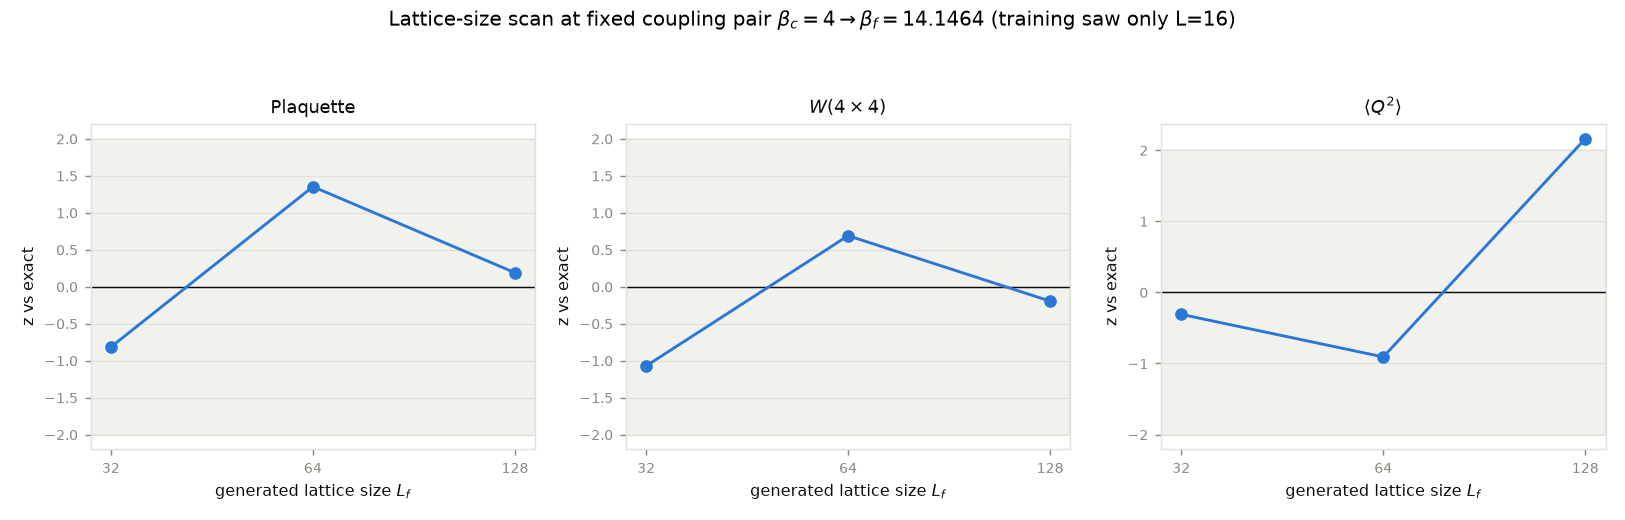
\includegraphics[width=0.9\linewidth]{figures/06_size_scan.png}
  \caption{\textbf{Volume transfer (part C).} The same checkpoint applied at
  $L = 64$ and $L = 128$ (never trained above $L = 32$); observables
  against exact values at $\beta_f = 14.15$. The v2 per-site normalization
  removes the lattice-size dependence that GroupNorm statistics introduced
  in earlier checkpoints.}
\end{figure}

\begin{figure}[p]
  \centering
  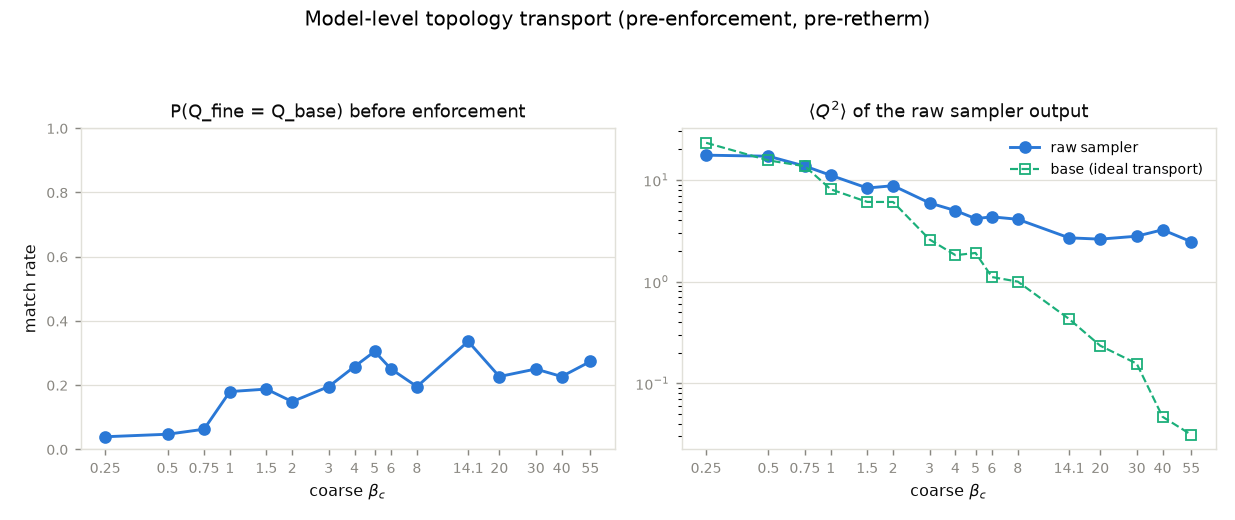
\includegraphics[width=0.9\linewidth]{figures/07_raw_topology.png}
  \caption{\textbf{Raw (pre-enforcement) topology transport.} The
  model-level metric charge enforcement would otherwise hide: spurious raw
  $\langle Q^2 \rangle$ excess over the coarse base, per track. v2's
  symmetry augmentation (charge conjugation ties the $\pm Q$ sectors) cuts
  the mean excess from 5.3 (v6) to 2.9, with the largest gains at low
  $\beta$ (e.g.\ $+11.3 \to +1.5$) --- under the stricter no-$Q$-hop
  rethermalization.}
\end{figure}

\begin{figure}[p]
  \centering
  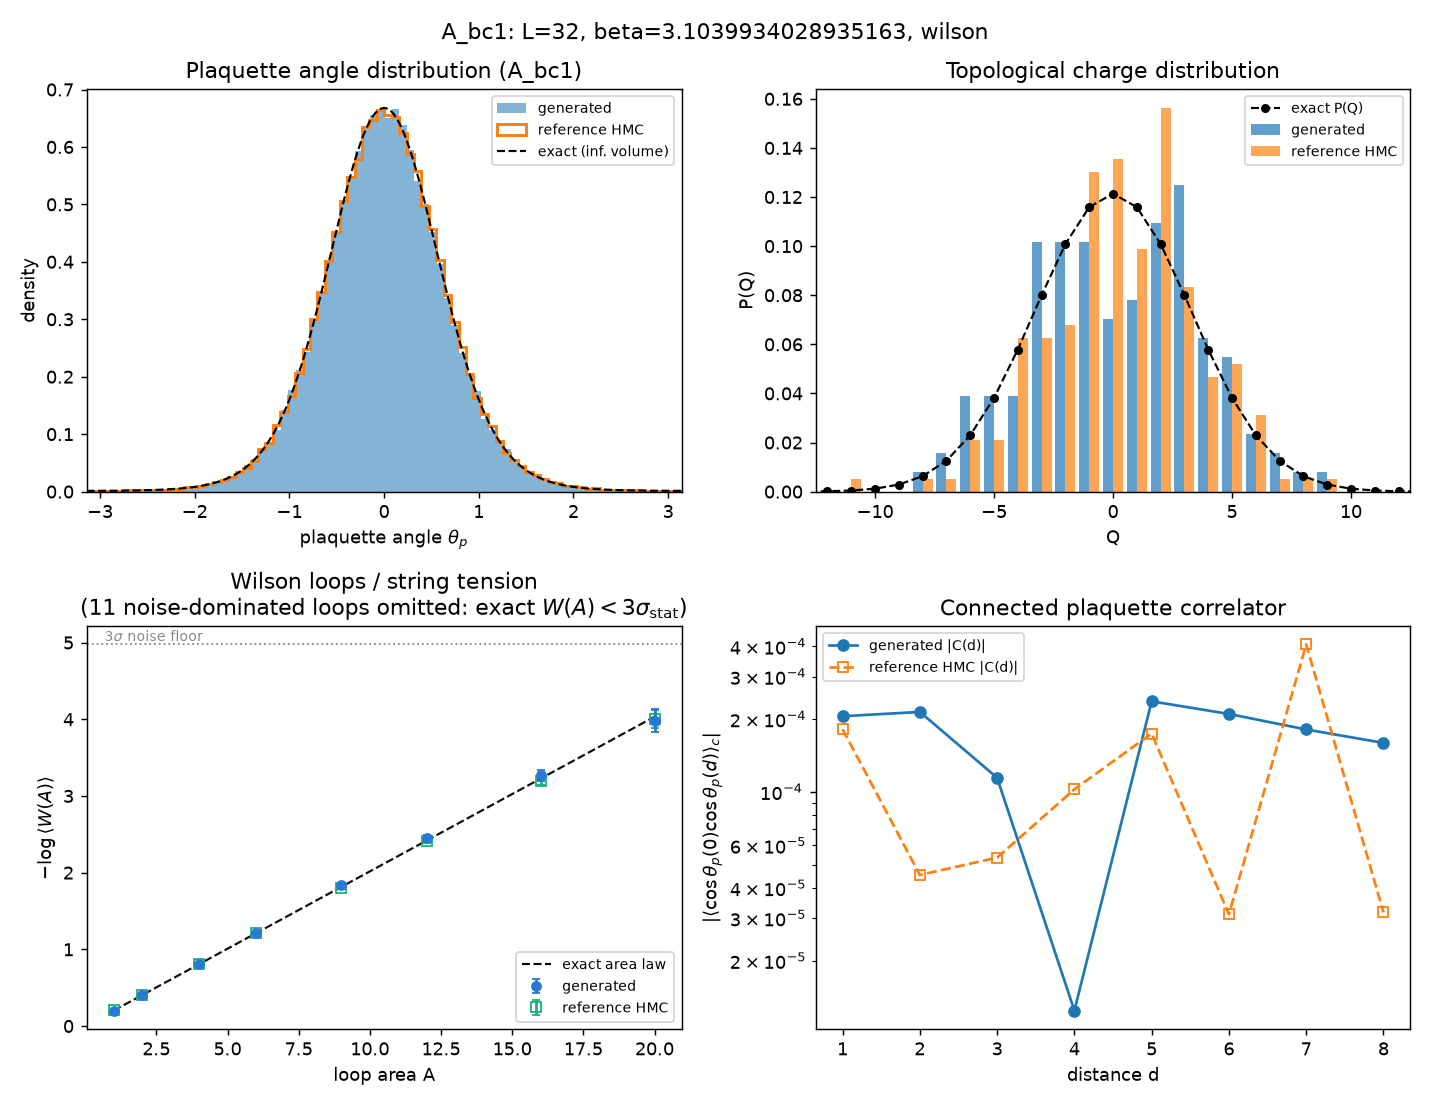
\includegraphics[width=0.9\linewidth]{figures/08_case_low.png}
  \caption{\textbf{Representative low-$\beta$ case ($\beta_f = 3.10$,
  $L = 32$).} Full validation panel in the regime where topology fluctuates
  freely and HMC is healthy --- the pipeline must (and does) reproduce a
  broad $P(Q)$.}
\end{figure}

\begin{figure}[p]
  \centering
  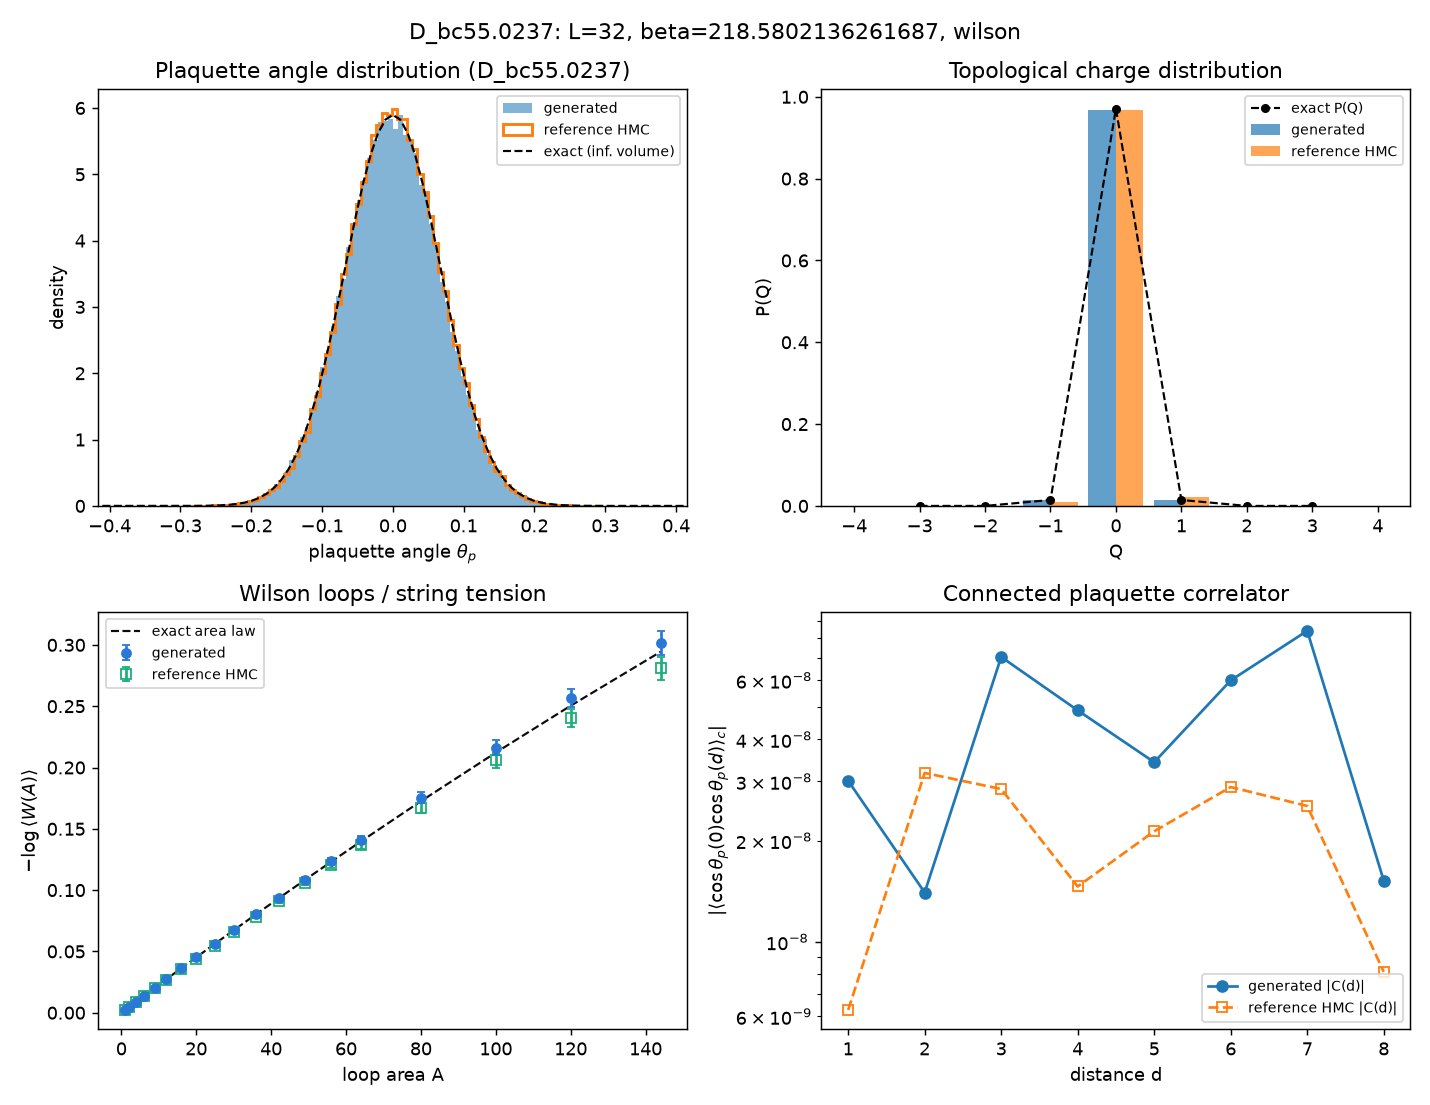
\includegraphics[width=0.9\linewidth]{figures/09_case_high.png}
  \caption{\textbf{Representative frozen-regime case ($\beta_f = 218.58$,
  $L = 32$).} Same panel deep in the topologically frozen regime (direct
  HMC: zero tunnelings). $\langle Q^2 \rangle$ agrees with the exact
  susceptibility; a fresh hot-start HMC ensemble at this coupling is wrong
  by two orders of magnitude in the same quantity.}
\end{figure}

\begin{figure}[p]
  \centering
  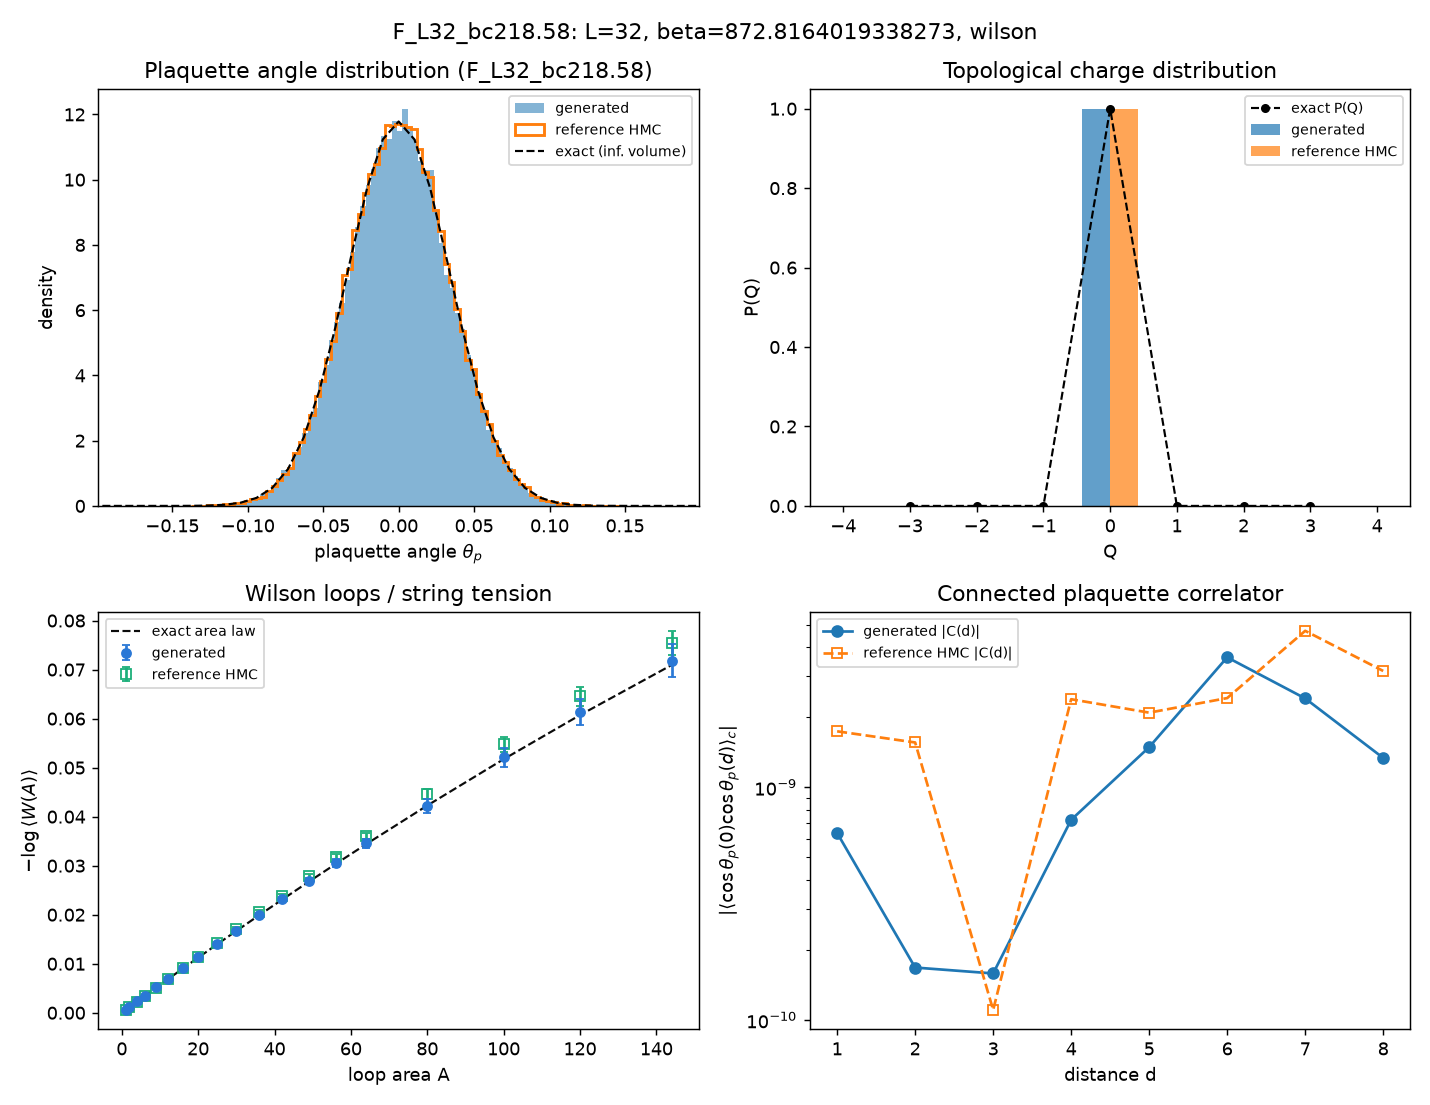
\includegraphics[width=0.9\linewidth]{figures/10_case_extrapolation.png}
  \caption{\textbf{Extrapolation frontier ($\beta_f = 872.8$, $L = 32$).}
  Fifteen times the training maximum. Wilson observables pass against exact
  values; exact $\langle Q^2 \rangle \approx 9\cdot 10^{-4}$ is consistent
  with the generated ensemble's (all-zero) charge content.}
\end{figure}

\begin{figure}[p]
  \centering
  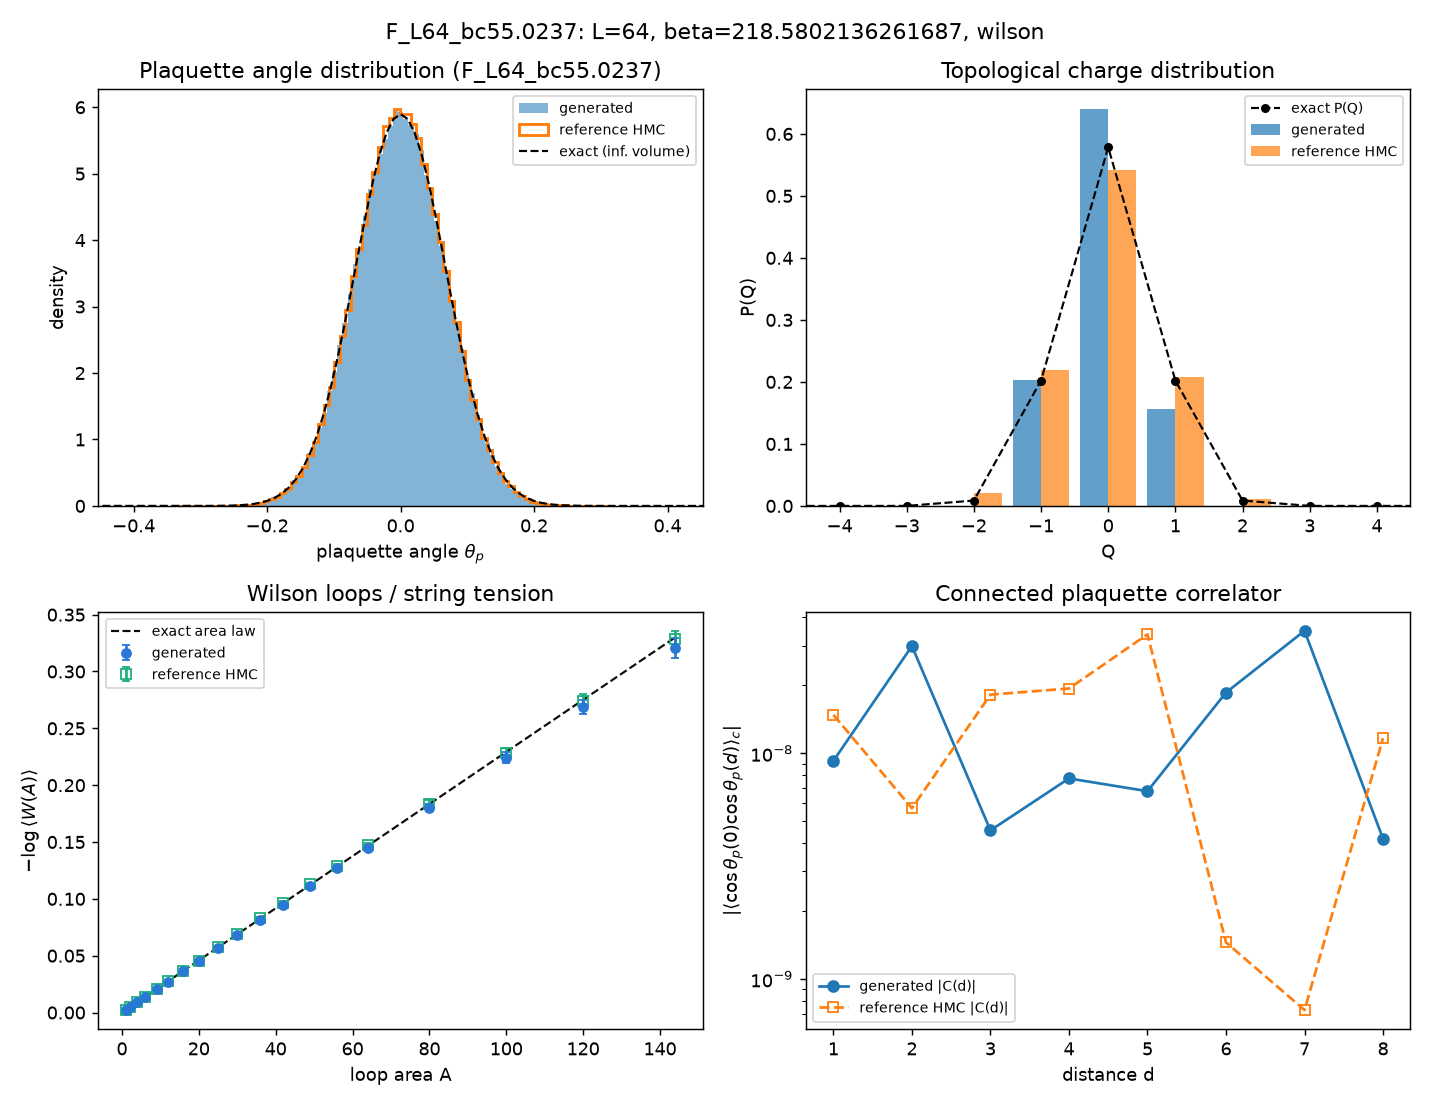
\includegraphics[width=0.9\linewidth]{figures/11_case_L64.png}
  \caption{\textbf{Joint coupling + volume extrapolation
  ($\beta_f = 218.58$, $L = 64$).} The hardest case in the study: $4\times$
  the training coupling and $4\times$ the training area simultaneously.}
\end{figure}

\begin{figure}[p]
  \centering
  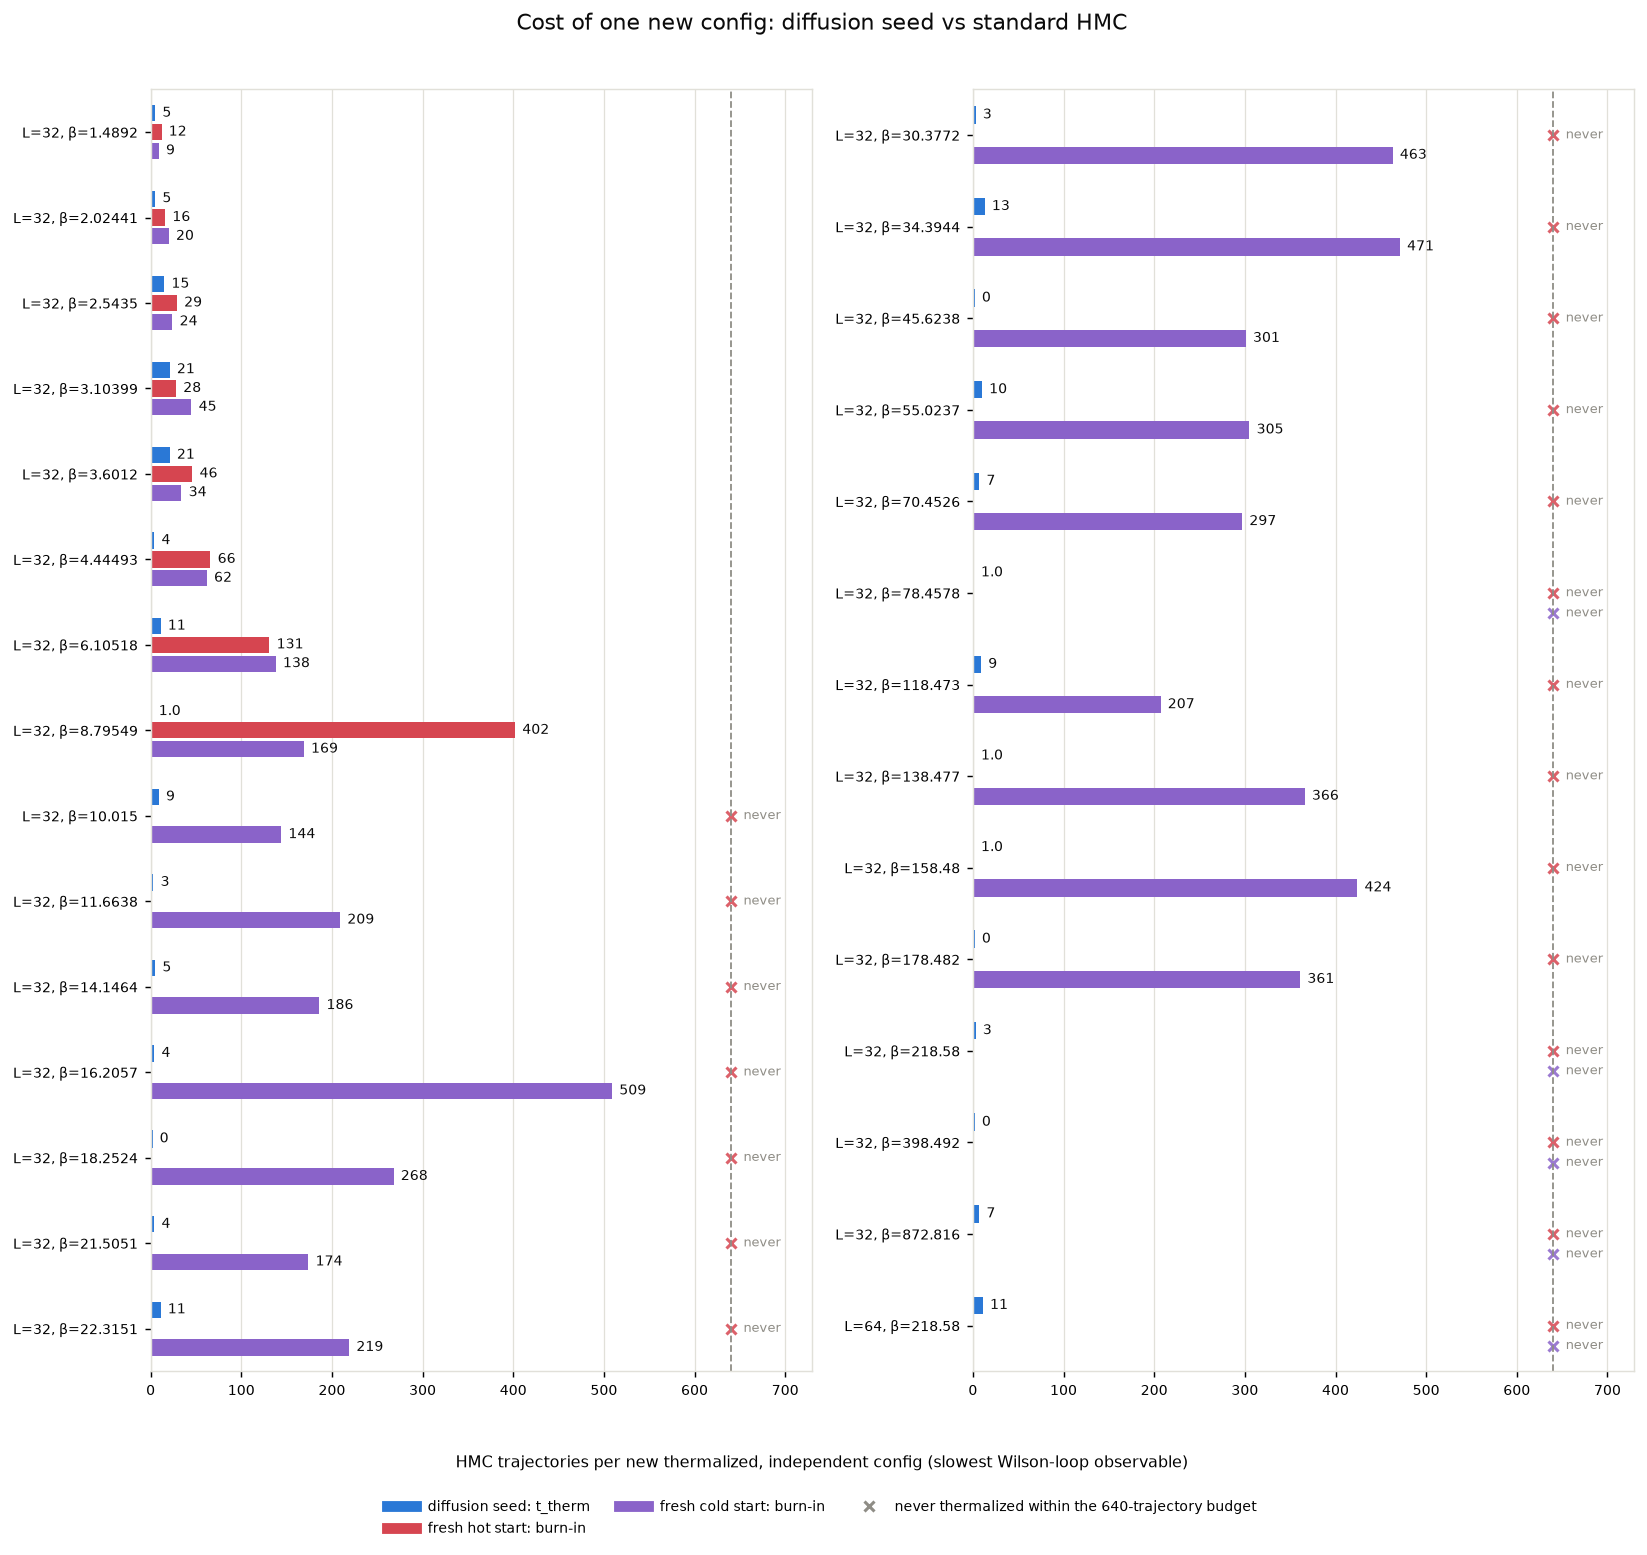
\includegraphics[width=0.9\linewidth]{figures/12_timescales.png}
  \caption{\textbf{Thermalization timescales.} Per coupling: $t_{\rm therm}$
  of an HMC chain started from a raw diffusion sample (no rethermalization
  applied --- every sweep the seed needs is charged here), the equilibrated
  chain's own sampling interval $2\tau_{\rm int}$, and fresh hot/cold-start
  burn-in. Seeds thermalize in 0--13 trajectories in 24 of 29 cases ---
  below the interval, i.e.\ cheaper than the chain's marginal cost per
  config; fresh hot chains never thermalize above $\beta \approx 8.8$.}
\end{figure}

\begin{figure}[p]
  \centering
  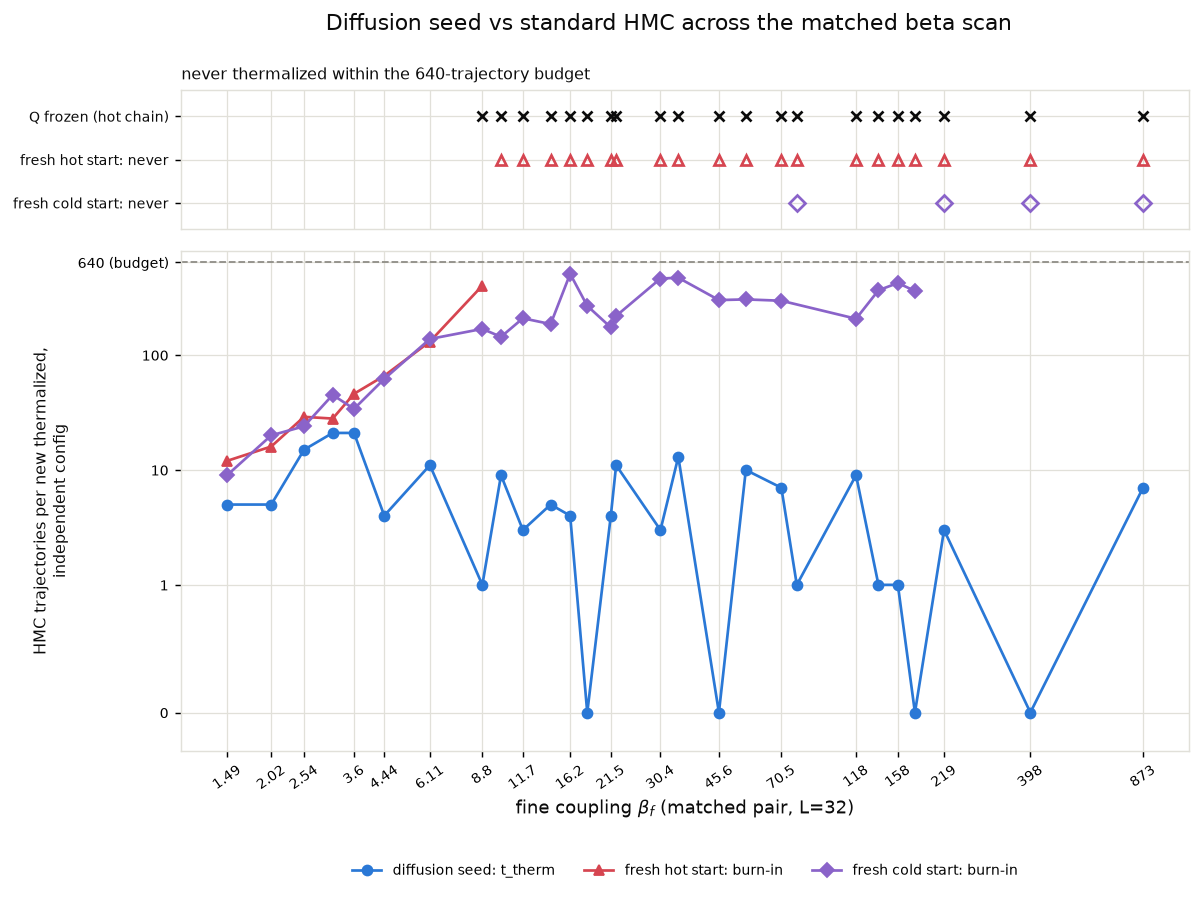
\includegraphics[width=0.9\linewidth]{figures/13_beta_scan.png}
  \caption{\textbf{Thermalization across the $\beta$ scan.} The same three
  quantities as a function of $\beta_f$: the ordering
  $t_{\rm therm}({\rm seed}) < 2\tau_{\rm int} < \text{burn-in(fresh)}$
  sets in at moderate coupling and widens as standard HMC slides into
  critical slowing down and topological freezing.}
\end{figure}

\begin{figure}[p]
  \centering
  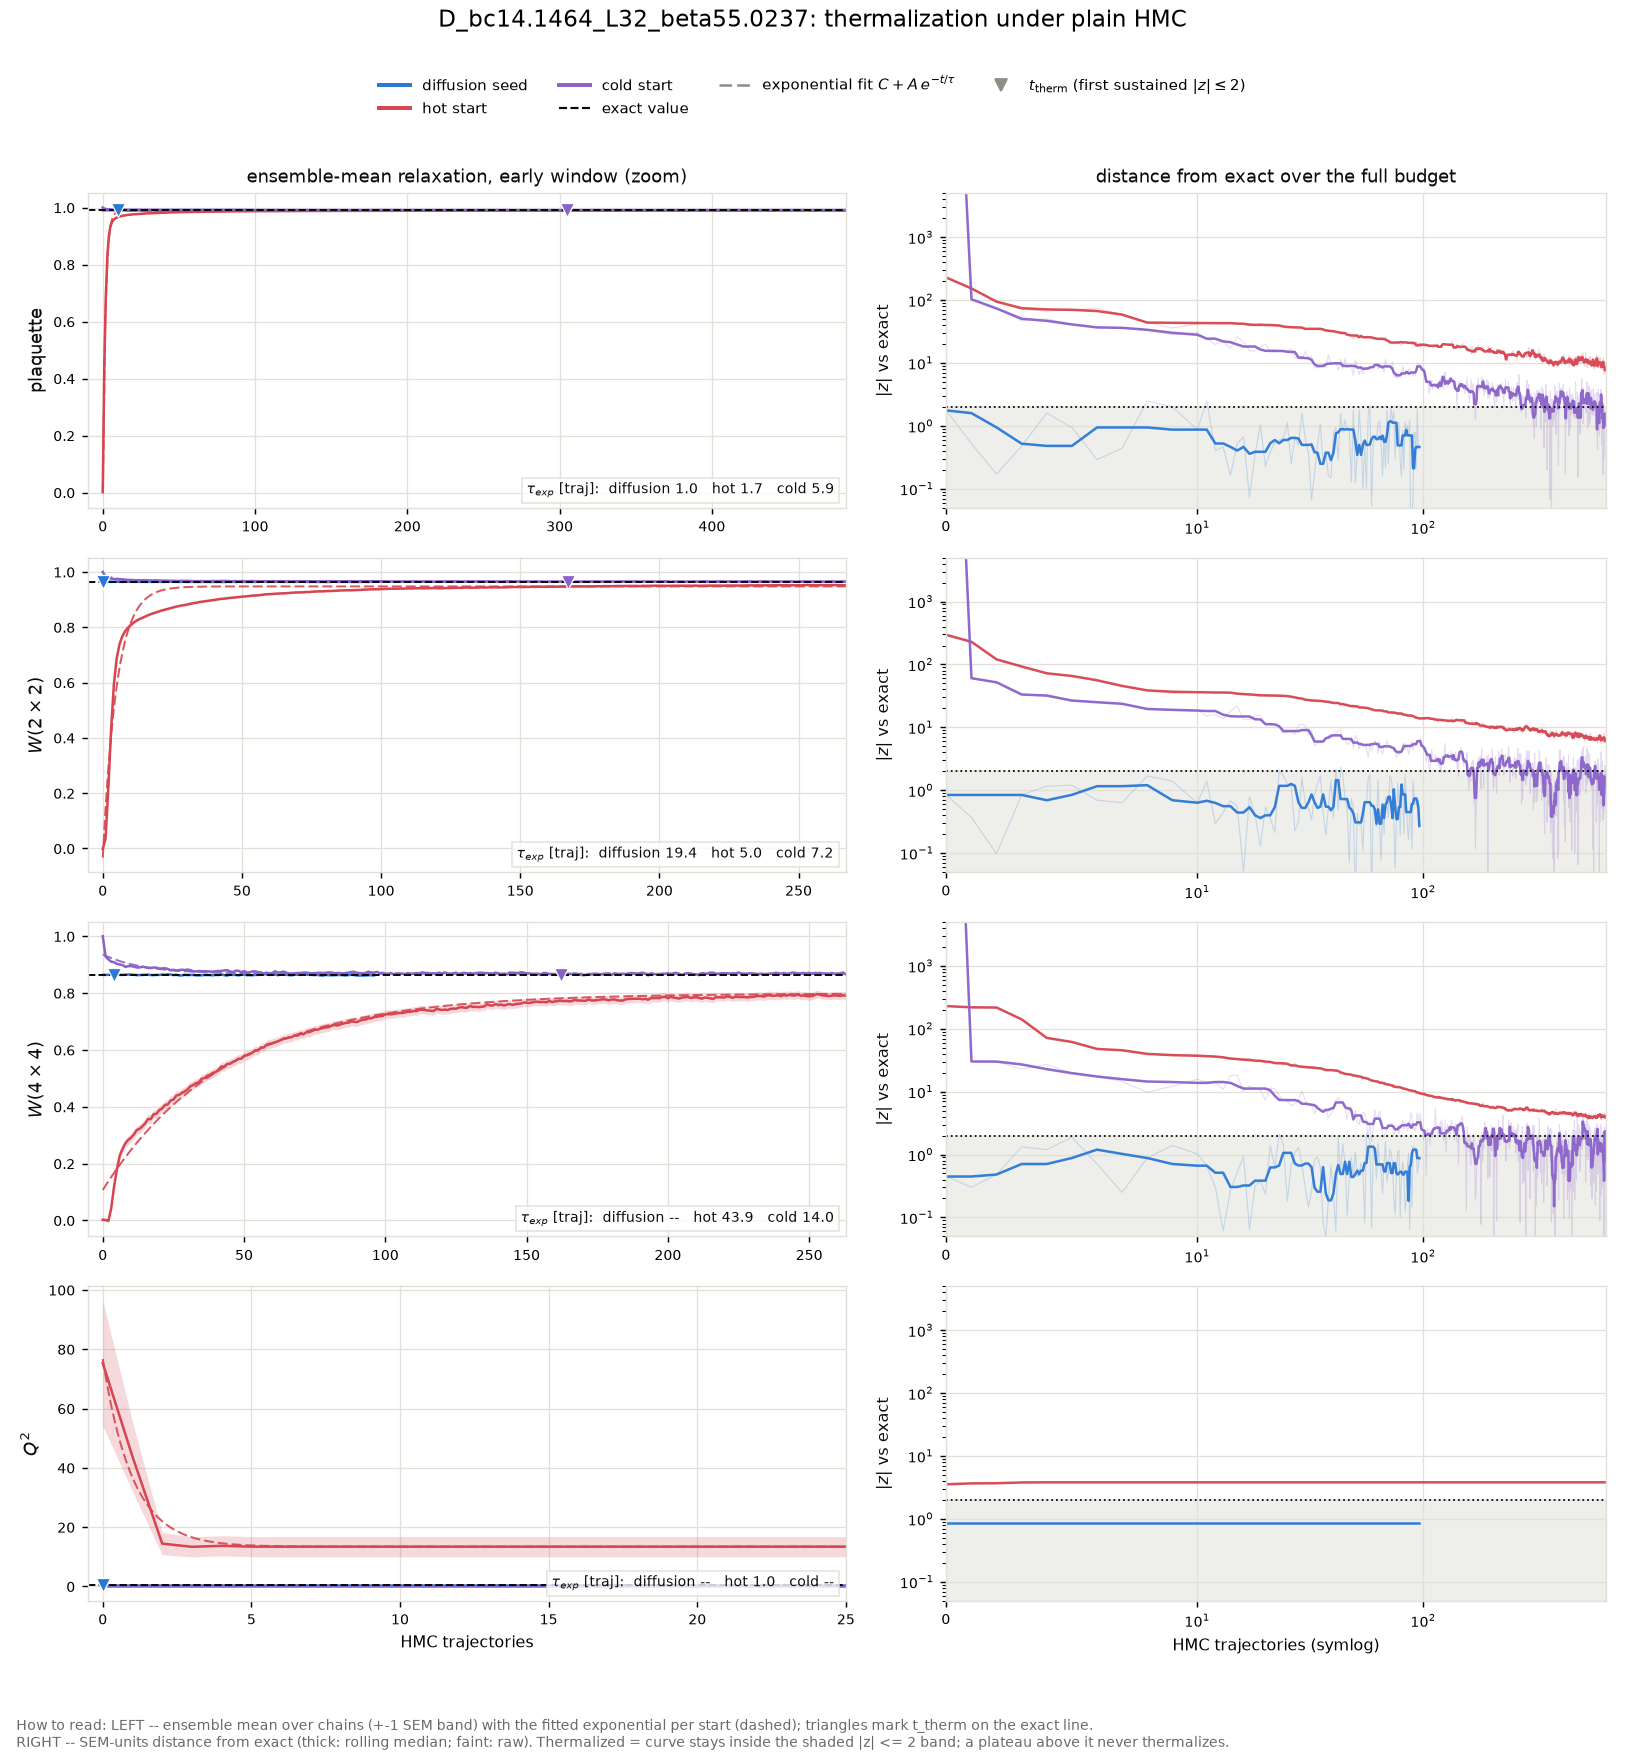
\includegraphics[width=0.9\linewidth]{figures/14_relaxation_mid.png}
  \caption{\textbf{Relaxation curves, $\beta_f = 55.02$ ($L = 32$).}
  Ensemble-mean observable traces for the three starting points with
  exponential fits and $|z| \le 2$ bands. The diffusion seed starts at its
  plateau (no measurable decay --- the desired outcome); hot and cold
  starts relax over hundreds of trajectories or not at all.}
\end{figure}

\begin{figure}[p]
  \centering
  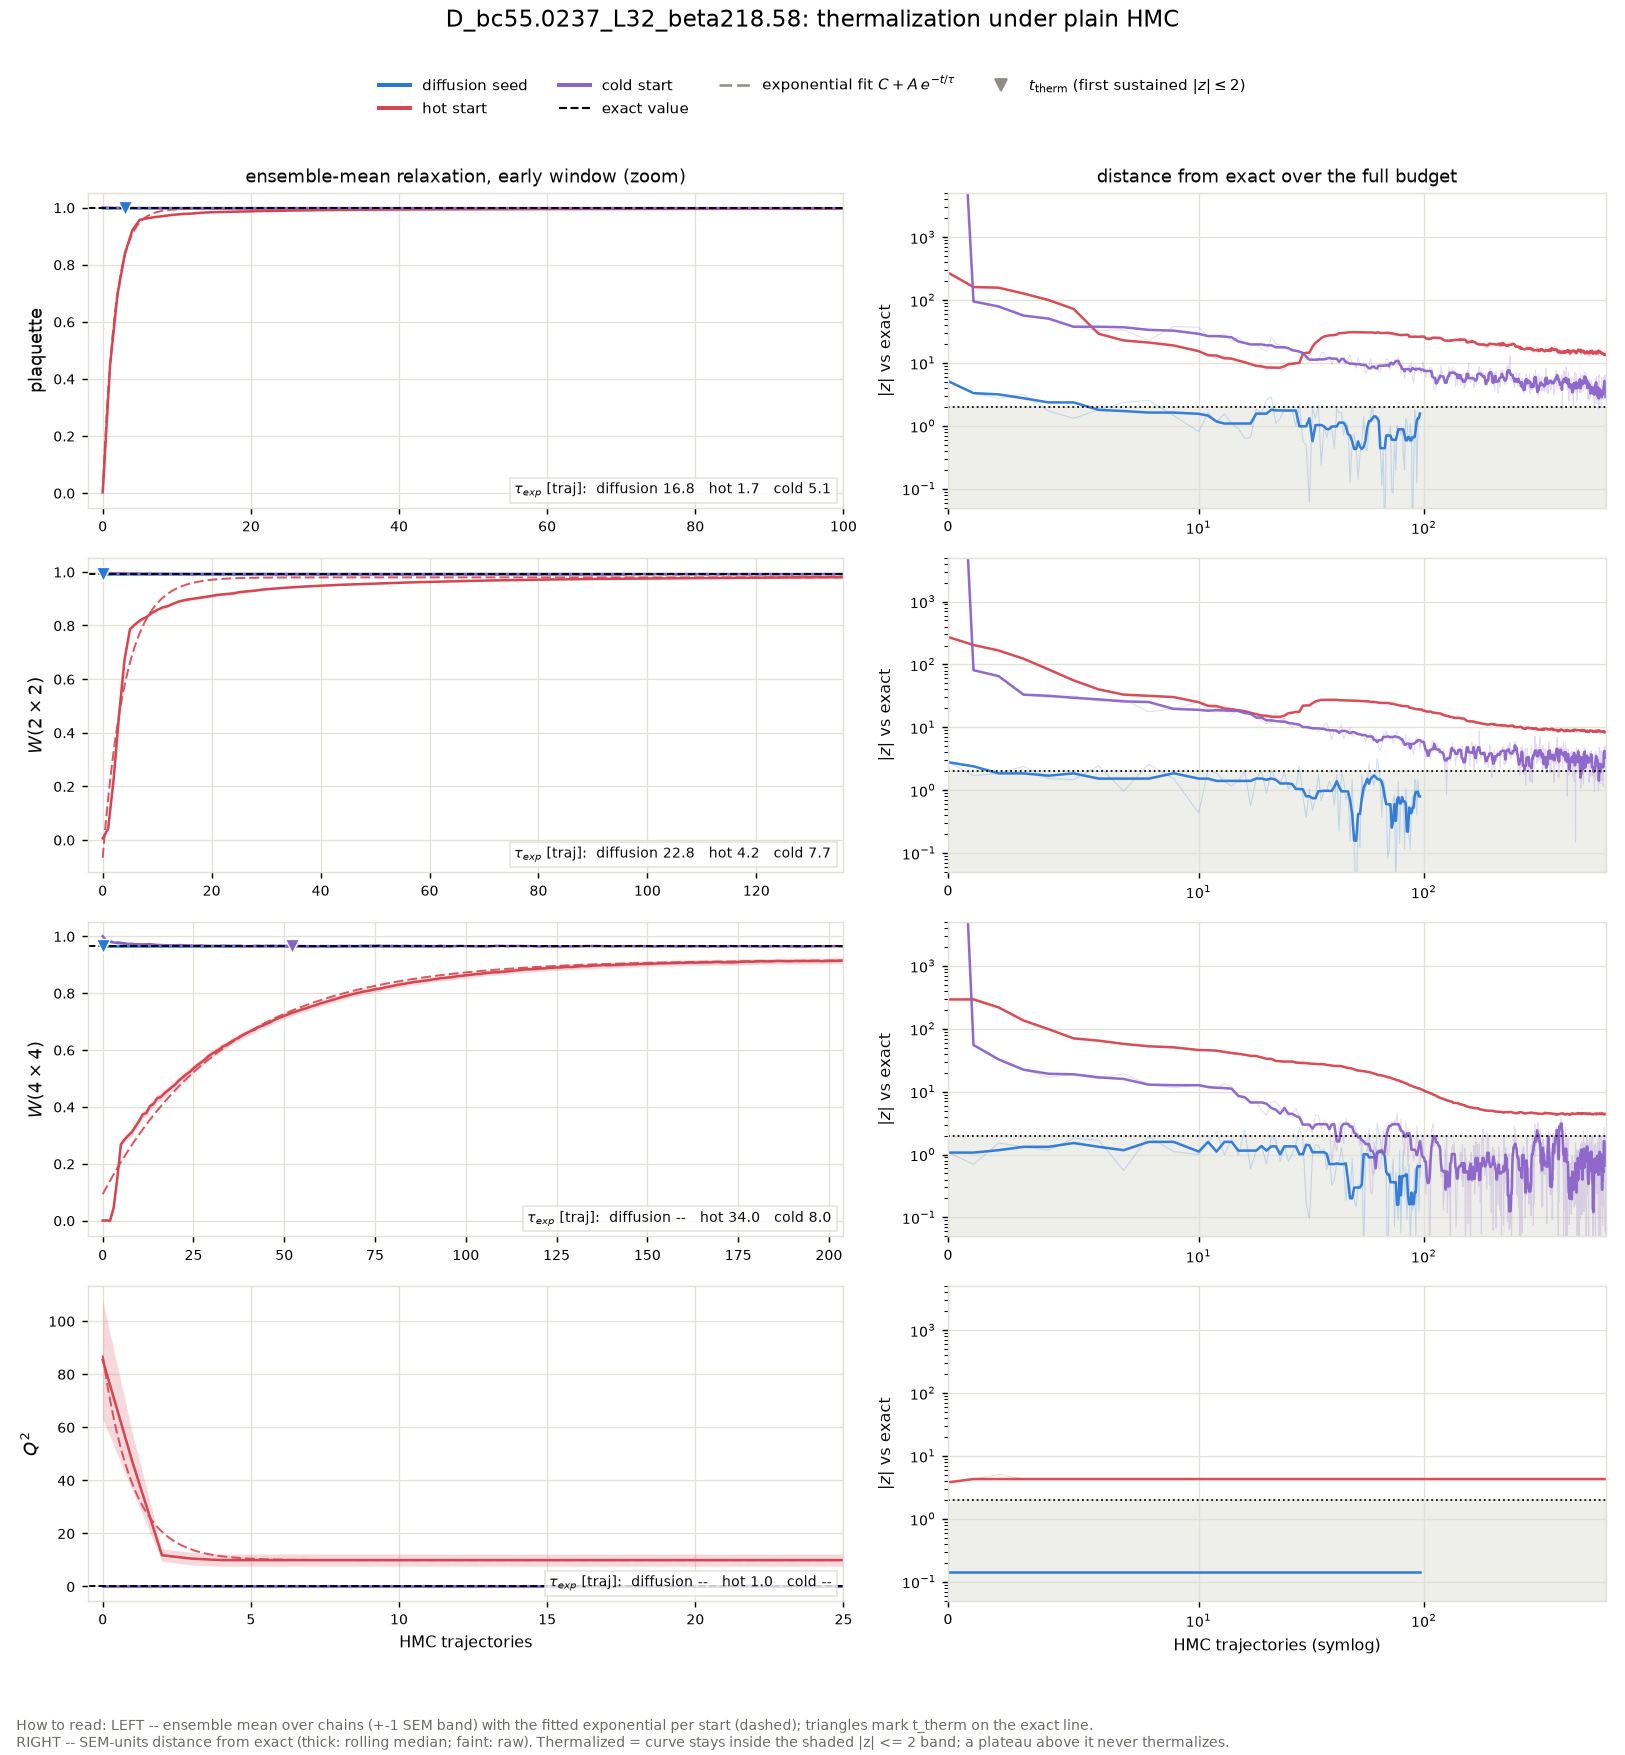
\includegraphics[width=0.9\linewidth]{figures/15_relaxation_high.png}
  \caption{\textbf{Relaxation curves, $\beta_f = 218.58$ ($L = 32$).} Same
  as the previous figure at the frozen regime's deep end: fresh chains
  never reach tolerance within the 640-trajectory budget; the seeded chain
  is indistinguishable from equilibrium within a few trajectories.}
\end{figure}

\begin{figure}[p]
  \centering
  
\includegraphics[width=0.9\linewidth]{figures/16_autocorrelation_modes.png}
  \caption{\textbf{Fast vs slow modes.} Normalized autocorrelation
  $\Gamma(\delta)$ of Wilson observables (fast modes) against the
  topological charge (slow mode) on equilibrated windows. Wilson-loop
  correlations decay within ${\sim}10$ trajectories while $\Gamma_Q$ stays
  pinned at 1 --- the frozen-topology signature; nothing in the seeded
  continuation depends on $Q$ mixing afterward, since the sector is
  transported, not evolved.}
\end{figure}

\begin{figure}[p]
  \centering
  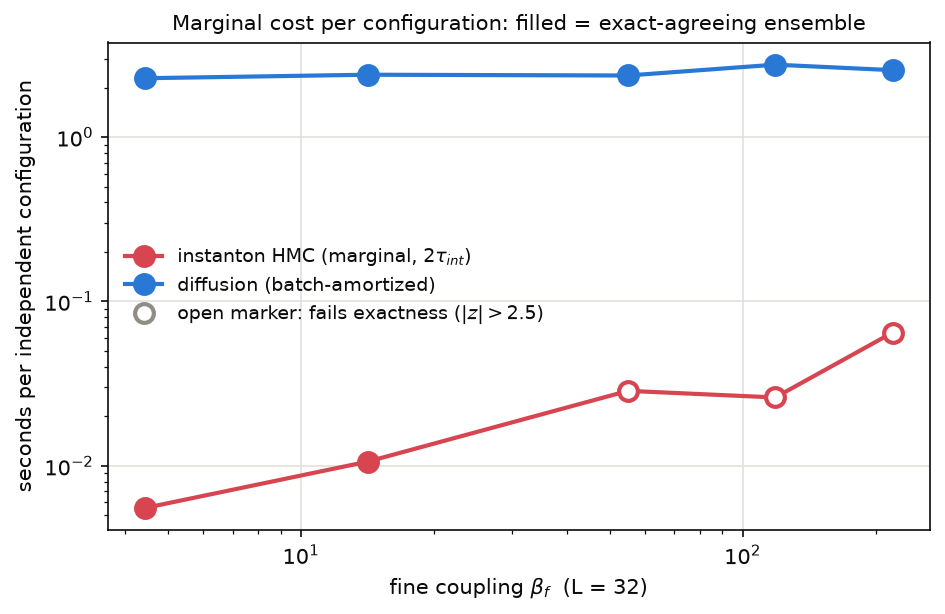
\includegraphics[width=0.85\linewidth]{figures/17_headtohead_cost.png}
  \caption{\textbf{Head-to-head vs instanton HMC: marginal cost and
  correctness ($L = 32$, burn-in 500, 128 configs/batch).} Instanton HMC
  --- the strongest classical baseline; its $Q$-hop keeps tunneling to
  $\beta = 256$ where standard HMC froze at 16 --- is far cheaper per
  config where it is correct (${\sim}0.01$\,s vs ${\sim}2.4$\,s), but open
  markers show it failing exactness (Wilson observables, up to $16.6\sigma$)
  at $\beta \ge 55$: its topology moves work, its UV does not thermalize.
  The diffusion pipeline passes everywhere at flat cost.}
\end{figure}

\begin{figure}[p]
  \centering
  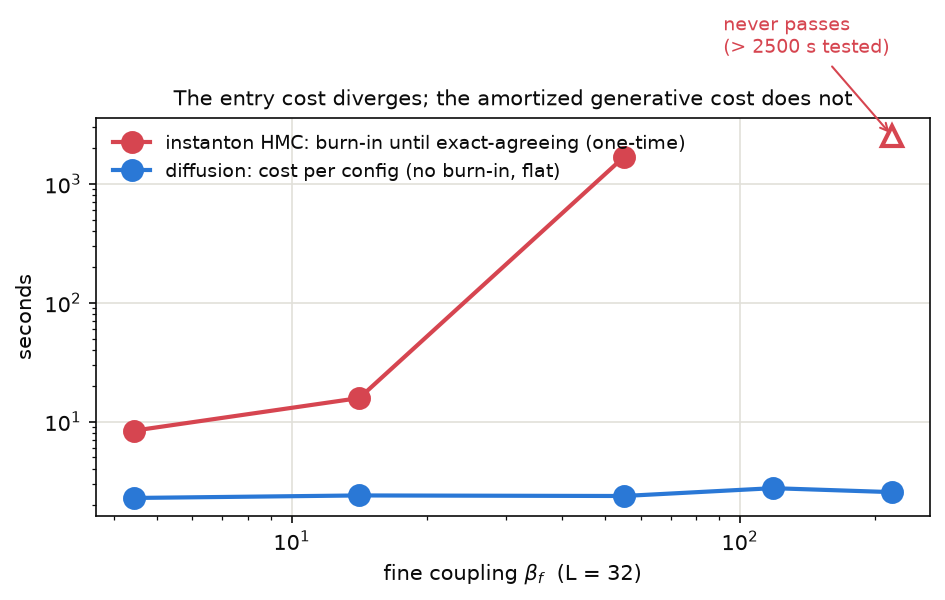
\includegraphics[width=0.85\linewidth]{figures/18_entry_cost.png}
  \caption{\textbf{Entry cost vs $\beta$ --- the head-to-head's decisive
  plot.} Burn-in wall-clock required before the instanton-HMC ensemble
  agrees with exact results: 8\,s ($\beta = 4.4$), 16\,s ($\beta = 14.1$),
  1677\,s ($\beta = 55$, needing 8000 trajectories), and \emph{never within
  the tested budget} at $\beta = 218.58$ ($7.2\sigma$ off after 8000
  trajectories / 2534\,s). The diffusion pipeline has no burn-in; its
  per-config cost is flat (2.3--2.8\,s) across the same range. The
  baseline's entry cost grows ${\sim}200\times$ over one decade of $\beta$
  and then stops converging; the generative cost does not.}
\end{figure}

\begin{figure}[p]
  \centering
  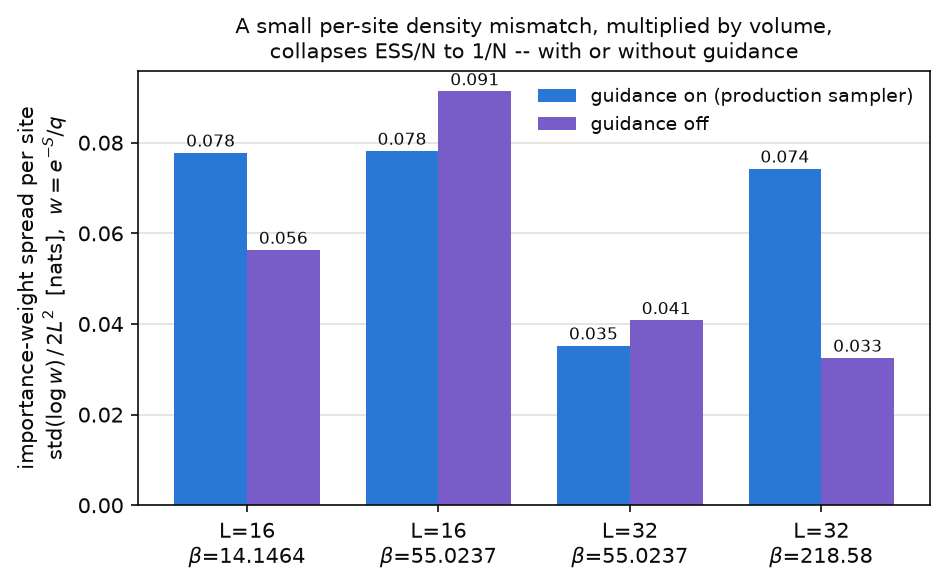
\includegraphics[width=0.85\linewidth]{figures/19_ess_weights.png}
  \caption{\textbf{Exact-likelihood diagnostic (honest negative).}
  Importance weights $w = e^{-S}/q$ from the probability-flow ODE
  likelihood (Hutchinson divergence, validated on an exactly solvable
  wrapped-Gaussian case), with the coarse-level density divided out via the
  matched-coupling action. The per-site weight spread is small
  (0.03--0.09 nats) but multiplies with volume, so ${\rm ESS}/N$ sits at
  the $1/N$ floor at $L = 32$ --- with the guidance term on or off,
  locating the gap in the score model's own density. The pipeline's
  correctness therefore rests on structural charge transport,
  rethermalization, and observable-level validation rather than
  reweighting; flow-based samplers with ${\rm ESS}/N \approx 0.5$--$0.7$
  hold that ground, while this pipeline's advantages are flat-cost seeding,
  extrapolation reach, and one-checkpoint generality. Closing the gap would
  require likelihood-aware training.}
\end{figure}

% -------------------------------------------------------------------

\begin{table}[p]
  \centering
  \caption{Instanton-HMC burn-in scan: entry cost vs quality at $L = 32$.
  Production window 640 trajectories $\times$ 32 chains throughout;
  quality = all Wilson-observable $|z| \le 2.5$ vs exact. Instanton-HMC
  $\langle Q^2 \rangle$ is correct in every row (the $Q$-hop works); the
  failures are UV thermalization.}
  \label{tab:burnin-scan}
  \begin{tabular}{rrrlrr}
    \toprule
    $\beta_f$ & burn-in & max Wilson $|z|$ & quality & entry cost (s) &
    diffusion s/config \\
    \midrule
    4.44   & 500  & 2.5  & pass & 8    & 2.28 \\
    14.15  & 500  & 1.7  & pass & 16   & 2.39 \\
    55.02  & 500  & 7.1  & fail & 31   & 2.37 \\
    55.02  & 2000 & 3.3  & fail & 328  & --   \\
    55.02  & 8000 & 1.1  & pass & 1677 & --   \\
    118.5  & 500  & 9.4  & fail & 42   & 2.76 \\
    218.58 & 500  & 16.6 & fail & 58   & 2.55 \\
    218.58 & 2000 & 7.8  & fail & 605  & --   \\
    218.58 & 8000 & 7.2  & fail & 2534 & --   \\
    \bottomrule
  \end{tabular}
\end{table}

\begin{table}[p]
  \centering
  \caption{Probability-flow ODE ESS of raw model transport. Guidance-off
  control: 0.019--0.021 at $L = 16$, 0.016 at $L = 32$ --- statistically
  identical, attributing the gap to the score model rather than the
  guidance terms.}
  \label{tab:ode-ess}
  \begin{tabular}{rrrr}
    \toprule
    $L$ & $\beta_f$ & ${\rm ESS}/N$ (fiber-corrected) &
    $\log w$ spread per site (nats) \\
    \midrule
    16 & 14.15  & 0.016 & 0.078 \\
    16 & 55.02  & 0.016 & 0.078 \\
    32 & 55.02  & 0.016 & 0.035 \\
    32 & 218.58 & 0.016 & 0.074 \\
    \bottomrule
  \end{tabular}
\end{table}
